\section{Background and Observation} \label{sec:background}
This work mainly relies on top of an SCGRA overlay based FPGA 
compilation. Thus both the overlay and the compilation 
framework are introduced in this section. In addition, 
we performed a number of experiments to show the 
predictable overlay characteristics such as performance 
hardware overhead, power and implementation frequency, 
and these characteristics contribute to the proposed design space exploration 
and customization framework. 

\subsection{SCGRA Overlay Compilation}
The SCGRA overlay based FPGA compilation framework 
is developed particularly for the sake of design productivity \cite{scgra}. 
With a pre-built overlay, it can produce an FPGA implementation 
in the order of seconds.

\figref{fig:scgra-compile} summarizes the SCGRA overlay 
compilation framework. It targets a CPU-FPGA system and includes 
two paths corresponding to software and hardware compilation flows. 
The path marked with green arrows represents the conventional software 
compilation flow and the final product is the binary code targeting the host CPU. 
The path marked with orange arrows shows the 
SCGRA overlay based accelerator compilation flow. It compiles a 
nested loop compute kernel to a data flow graph (DFG) and then schedules 
the DFG to the specified SCGRA through an operation scheduler. 
The scheduling result can then be embedded directly into the pre-implemented 
SCGRA overlay to produce the final FPGA configuration bitstream.

\begin{figure}[H]
\center{\includegraphics[width=0.8\linewidth]{framework}}
\caption{SCGRA Overlay Compilation Framework}
\label{fig:scgra-compile}
\end{figure}

\begin{figure}[H]
\center{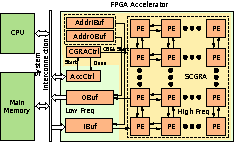
\includegraphics[width=0.8\linewidth]{scgra-accelerator}}
\caption{SCGRA Overlay Based FPGA Accelerator}
\label{fig:scgra-acc}
\end{figure}

\figref{fig:scgra-acc} shows the design of a typical SCGRA overlay 
based FPGA accelerator. In the accelerator, on-chip
memory i.e. IBuf and OBuf are used to buffer data between the host CPU and 
the accelerator. A controller is also presented in hardware 
to control the operations of the accelerator as well as
memory transfers. The SCGRA, which is the kernel computation fabric,
consists of an array of processing elements 
(PEs) and it achieves the computation 
task through the distributed control words stored in each PE. The AddrBuf 
stores all the valid IO buffer accessing addresses of the DFG while 
the valid signals come from the BitMapper. In order 
to amortize the IO data transmission cost, we may group a number of 
DFG and have the IO transmitted in the granularity of a group. Accordingly,
AddrBuf should store all the addresses of the group while the control words 
in each PE can still be reused.

\subsection{Predictivity of SCGRA Overlay}
In order to simplify the customization, we have performed 
a series of experiments on Zedboard \cite{zedboard} to 
analyze how different design parameters affect the 
performance, power and overhead. 

\figref{fig:perf-influence} shows the influence of SCGRA size and 
unrolling factor on the execution time of a loop kernel. Although there 
are slightly variation when the extracted DFG or the unrolling 
factor is small, both parameters basically present monotonic impact on 
the execution time.

\begin{figure}[H]
    \subfloat[\label{fig:scgrasize-perf}]{%
      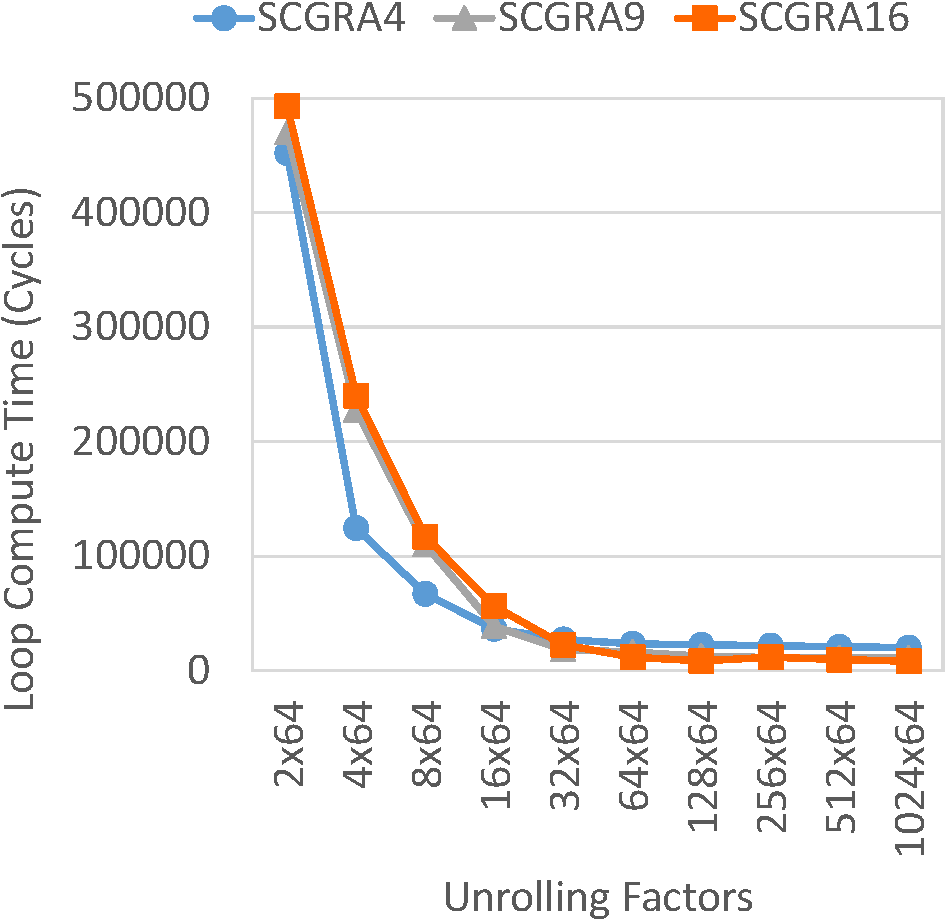
\includegraphics[width=0.23\textwidth]{scgrasize-perf}
    }
    %\hfill
    \subfloat[\label{fig:unrolling-perf}]{%
      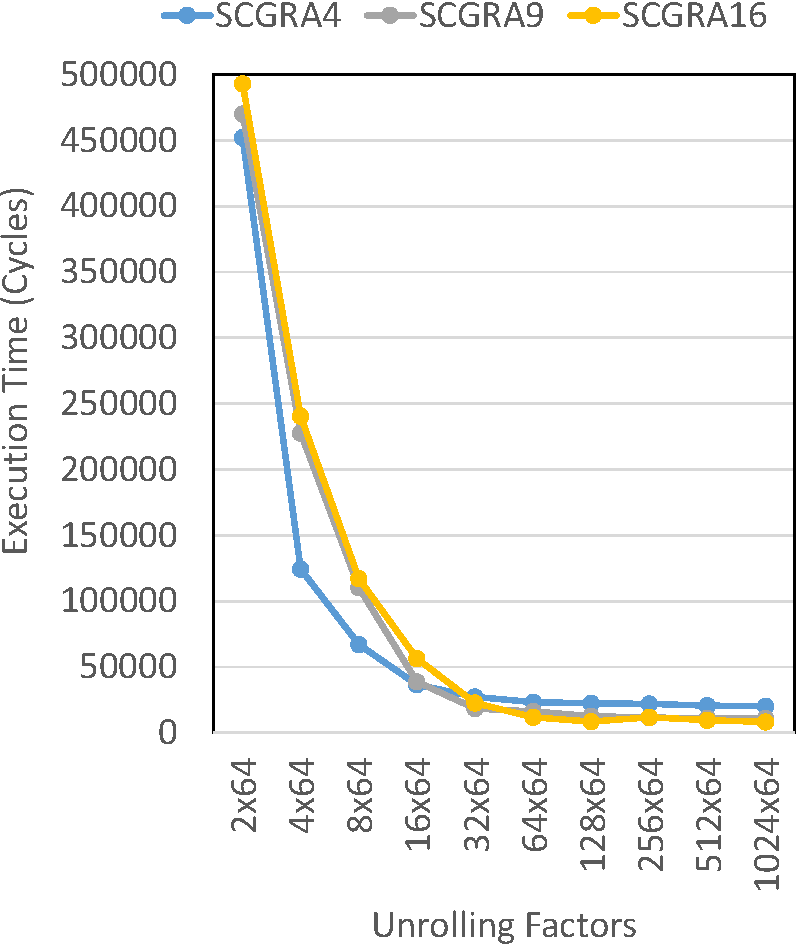
\includegraphics[width=0.24\textwidth]{unrolling-perf}
    }
    \caption{Design Parameter Influence on Execution Time, (a) SCGRA Size, (b) Unrolling
    Factor}
    \label{fig:perf-influence}
  \end{figure}


\figref{fig:scgra-overhead} shows the overhead, implementation 
frequency and power of a group of SCGRA overlay implementation.
The basic configuration is listed in \tabref{tab:config}. According to this 
figure, it is found that the results typically present good 
linearity over the SCGRA overlay size and therefore simple models can be used 
to achieve an adequate estimation.
\begin{table}[H]
  \caption{Experiment Configuration \label{tab:config}}{
  \centering
  \begin{tabular}{l|l|l|l|l}
  \hline
  DataWidth & InstRom & DataMem & IBuf/OBuf & AddrBuf \\ \hline
  32 & 1kx72bit & 256 & 2048 & 4kx16bit\\ \hline
  \end{tabular}
  }
\end{table}

\begin{figure}[H]
    \subfloat[\label{fig:scgrasize-impl}]{%
      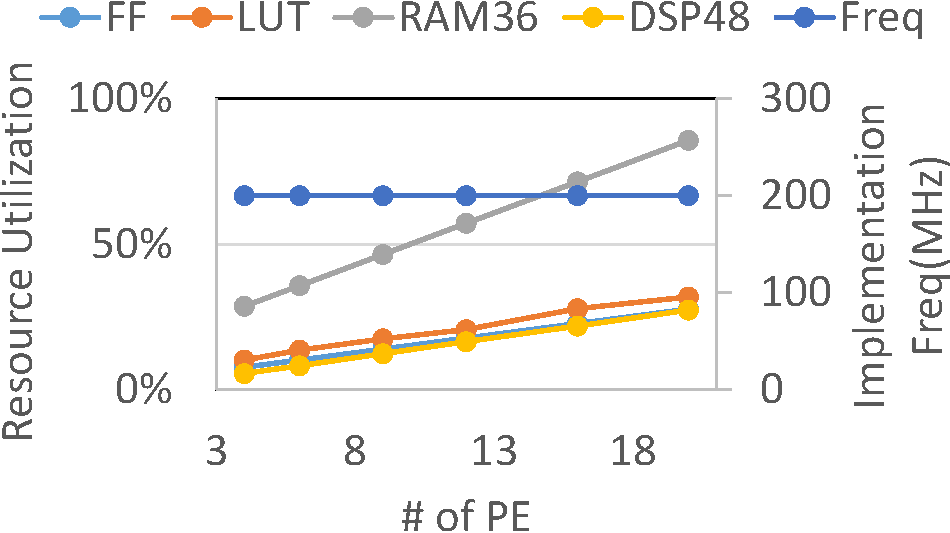
\includegraphics[width=0.24\textwidth]{scgrasize-impl}
    }
    %\hfill
    \subfloat[\label{fig:scgrasize-power}]{%
      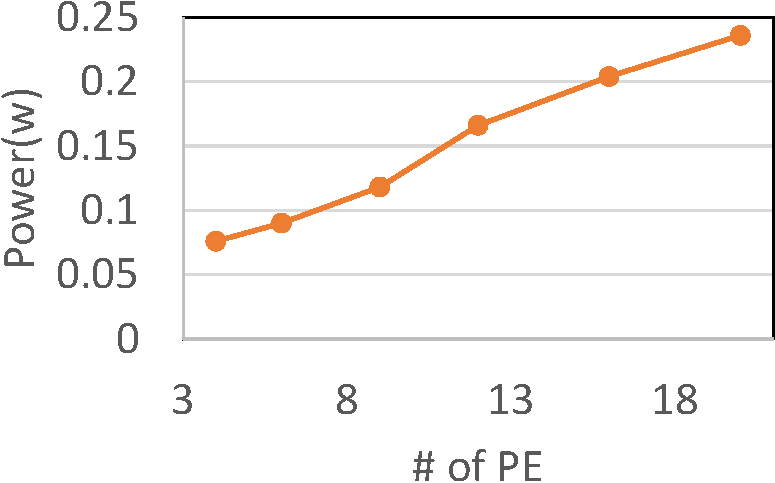
\includegraphics[width=0.2\textwidth]{scgrasize-power}
    }
    \caption{SCGRA Overlay Overhead and Power, (a) Overhead, (b) Power}
    \label{fig:scgra-overhead}
\end{figure}

